\documentclass[12pt]{article}
\usepackage[a4paper,left=1in,right=1in,top=1in,bottom=1in]{geometry}
\usepackage[utf8x]{inputenc}
\usepackage{textcomp,gensymb}
\usepackage{indentfirst}
\usepackage{graphicx}
\graphicspath{{/home/dnehme/Dropbox/profissional/protocolos/ptc-validation-roms/ssh/figure/}}
\usepackage[abs]{overpic}
\usepackage{float}
\usepackage[brazil]{babel}
\usepackage{multirow}
\usepackage{lmodern}
\usepackage{titlesec}
\usepackage{xcolor}
\usepackage{natbib}
\usepackage{hyperref}

\setcounter{secnumdepth}{4}

\titleformat{\paragraph}
{\normalfont\normalsize\bfseries}{\theparagraph}{1em}{}
\titlespacing*{\paragraph}
{0pt}{3.25ex plus 1ex minus .2ex}{1.5ex plus .2ex}


\begin{document}

\begin{center}
	{\bf {\Large Protocolo de validação de simulações do ROMS}}
	\vspace{5mm}\par

	{\bf {\large Elevação da Superfície Livre do Mar}}
	\\
	\hrulefill
	\\
	
	{\bf Equipe:} {\it Douglas M. Nehme}\\
	\par
\end{center}

\tableofcontents

\newpage

\addcontentsline{toc}{section}{Apresentação}
\section*{Apresentação}
	\par Este protocolo descreve o processo de validação dos resultados de elevação da superfície livre do mar de simulações do ROMS usando dados de altimetria por satélite produzidos pelo \textit{Data Unification and Altimeter Combination System} (DUACS), que está inserido no segmento de apoio terrestre a instrumentos em órbita (SSALTO, em francês) da agência espacial francesa (CNES, em francês). Até abril de 2017, este e os demais produtos produzidos pelo DUACS/SSALTO eram distribuidos pelo portal \textit{Archiving, Validation and Interpretation of Satellite Oceanographic data} (AVISO) e atualmente estão integrados à base de dados do \textit{Copernicus Marine Environment Monitoring Service} (CMEMS), que é o componente marinho do progrma de observação da Terra da União Europeia (Copernicus).
	
\section{Variáveis obtidas por satélite}
	\label{sec:variaveis_satelitais}
	\par Antes de descrever as variáveis possíveis de serem calculadas a partir das medidas feitas pelos altímetros é importante saber que a altitude em que um satélite se encontra é definida em relação ao elipsóide de referência e os altímetros medem a variação altimétrica, que é a distância de seu centro de massa à superfície da Terra, como representado na Figura \ref{fig:variaveis_altimetria}. Nesta figura, além do elipsóide de referência, que é uma aproximação da crosta terrestre de forma esférica com os pólos achatados, retrata-se o geóide, que é a superfície que o oceano assumiria na ausência de forças, como os ventos, correntes ou marés. O geóide terestre reflete o campo gravitacional do nosso planeta e é uma superfície equipotencial.
	\par Na altimetria por satélite as medidas de interesse para a oceanografia são aquelas ligadas à porção dinâmica do sinal, pois são essas variações que efetivamente se relacionam com os forçantes termodinâmicos que colocam o oceano em movimento e modificam o geóide. Por isso as variáveis de interessem tem como superfície de referência o geóide em detrimento do elipsóide.

	\begin{figure}[H]%[h!]
		\centering
		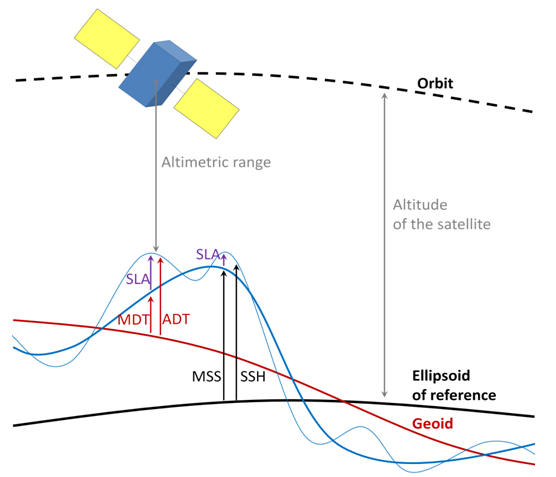
\includegraphics[width=0.8\textwidth]{ABC_Altimetry.png}
   		\caption{Representação esquemática das diferentes variáveis e superfícies de referência utilizadas na altimetria por satélite \citep{taburet_etal2021}. Variáveis descritas ao longo da Seção \ref{sec:variaveis_satelitais}.
    	\label{fig:variaveis_altimetria}}
	\end{figure}
	
	\par A seguir são definidas as variáveis apresentadas na Figura \ref{fig:variaveis_altimetria}.

	\begin{itemize}
		\item Elevação da Superfície Livre do Mar\footnote[1]{Dependendo da área da oceanografia a Elevação da Superfície Livre do Mar pode apresentar diferentes significados, sendo descrito neste protocolo o utilizado em altimetria por satélite.} (\textit{Sea Surface Height} - SSH): Altura da coluna d'água, em um instante qualquer, em relação ao elipsóide de referência, sendo calculada a partir da variação altimétrica medida pelo satélite.
		
		\begin{center}
			SSH = Altitude do Satélite - Variação Altimétrica - Correções\footnote[2]{Correções devido às condições ambientais}
		\end{center}
		
		\item Elevação Média da Superfície Livre do Mar (\textit{Mean Sea Surface} - MSS\textsubscript{N}): Média temporal da SSH calculada para um período N, conhecido como período de referência e que, habitual e prudentemente, representa diversos anos. Os produtos produzidos pelo DUACS/SSALTO possuem como N o intervalo de 20 anos entre 1993 a 2012. Se necessário for, \citet{pujol_etal2016} propõem uma metodologia para modificar o N.

		\[MSS_N = \frac{1}{N} \sum_{i=1}^{N} SSH_i \]	
		
		\item Anomalia da Superfície Livre do Mar (\textit{Sea Level Anomlay} - SLA\textsubscript{N}): Desvio do valor da SSH em torno da média (MSS\textsubscript{N}). Assim como a MSS\textsubscript{N} a SLA\textsubscript{N} varia de acordo com a definição do N.
		
		\begin{center}
			SLA\textsubscript{N} = SSH - MSS\textsubscript{N}
		\end{center}	
		
		\item Topografia Dinâmica Média (\textit{Mean Dynamic Topography} - MDT\textsubscript{N}): é a média temporal da SSH calculada para um período N, mas não tendo como referência o elipsóide, mas sim o geóide.
		
		\begin{center}
			MDT\textsubscript{N} = MSS\textsubscript{N} - Geóide
		\end{center}	
		
		\item Topografia Dinâmica Absoluta (\textit{Absolut Dynamic Topography} - ADT): Altura da coluna d'água, em um instante qualquer, em relação ao geóide. Como o desvio do estado de repouso do oceano representado pelo geóide fornece informações sobre a sua dinâmica, esta é a variável a partir da qual se calculam as correntes geostróficas. E assim como a SSH, a ADT é independente do período de referência. A ADT ainda não é passível de ser estimada através da subtração do geóide diretamente da SSH obtida pelo satélite, pois os dados do geóide não possuem acurácia capaz de representar estruras de menor escala ($\textless\approx{}$100km). Por isso, para obter informações das estruturas dinâmicas com menores comprimentos de onda este processo de cálculo é necessário.
		
		\begin{center}
			ADT = MDT\textsubscript{N} + SLA\textsubscript{N}
		\end{center}	
		
	\end{itemize}
	
	\par Dentre as cinco variáveis definidas anteriormente, duas se relacionam com o elipsóide (SSH e MSS\textsubscript{N}), duas com o geóide (ADT e MDT) e uma é independente (SLA\textsubscript{N}). Além disso, temos a SSH e a ADT como o sinal altimétrico total, a MSS\textsubscript{N} e a MDT como o sinal médio e a SLA\textsubscript{N} como o desvio ou a variabilidade.
	\par As informações presentes nesta seção se baseiam em \citet{rosmorduc_etal2018}, \citet{duacs_web_faq2021} e \citet{taburet_etal2021}.

\section{Variável gerada pelo modelo}
	\par A

\section{Comparação dos dados de satélite com os resultados do modelo}
	\par Além de descrever como é feita a comparação e quais variáveis são usadas, citar que o zeta do ROMS não é totalmente igual ao ADT por causa do efeito estérico da água, que é produzido por sua expansão térmica e não está presente em modelos que consideram a aproximação de Boussinesq.

\section{Produtos satelitais disponíveis}
	\par Falar dos prós e contras do produto Near Real Time e do Reprocessed que são a diferença entre tempo de latência e quantidade de dados utilizada.

\section{Download dos arquivos}
	\par A
	
\bibliographystyle{coppe-plain}
\typeout{}
\bibliography{biblio/biblio}
\addcontentsline{toc}{section}{Referências}

\end{document}
